\documentclass{article}

\usepackage[margin=1in,includefoot]{geometry}

\usepackage{graphicx}
\usepackage{hyperref}

\begin{document}
	\begin{titlepage}

	
	
\section{Project Statement}\label{sec intro}
The project is about Result Management System is to provide the examination result to the student in a simplified manner. This is useful for students to manage the results. 
The system is intended for the students and various functionalities are provided to students such as calculation of GPA, to read and execute student’s result by providing user name and password for secure login and in case of new student’s, the registration is available. Teacher’s  can easily calculate  the result  of any student. The whole result management system will be under the control of the administrator panel. 


\section{Objective}\label{sec intro}
a)	Information about the various Users \\
b)	Information about subjects offered in various semesters \\
c)	Marks obtain by Students in different semesters\\
d)	Generate/Download Report of all Results in PDF Format\\




\section{Working Hypothesis}\label{oject}

Hypothesis 1 : Our project is mainly based on data base. Here ,remain different access for COE office, Teachers  and  Students. \\
Hypothesis 2 : Student get CT marks , Assessment marks and Total marks easily by using this system. \\
Hypothesis 3 : In future , We will use SMS alert system for Guardian to get a result of a student.
\\

\label{oject}
Access point :

\begin{figure}[h!]
\centering
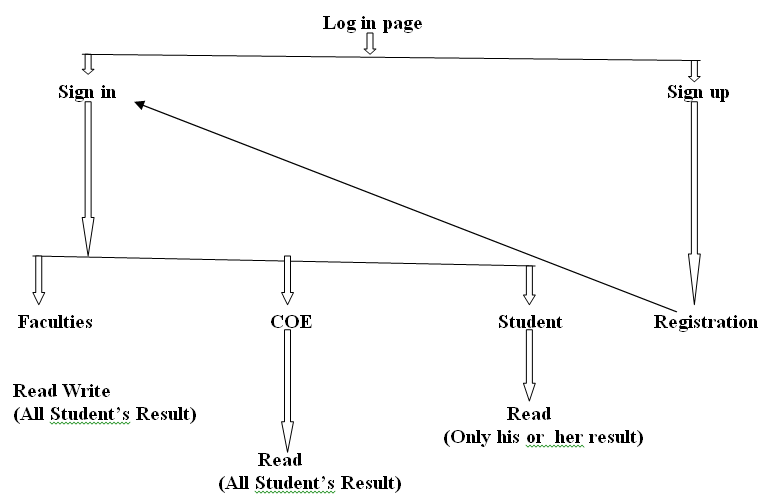
\includegraphics[width=.9\textwidth]{Access.png}

\end{figure}

\vspace{10cm}

\section{Tools}\label{oject}

Here, we use MYSQL for data base. HTML, CSS, JAVA SCRIPT for frontend design and LARAVEL for framework.


\section{References}\label{oject}
I.	Udemy Course Tutorial about HTML,CSS,JAVA SCRIPT,LARAVEL \\
II.	University course material: MYSQL \\
III. \url{https://www.youtube.com/results?search_query=coder+foundation} \\
IV. \url{https://www.youtube.com/channel/UCzmI_aDsHbBXPZzabrsM7sA}



\end{titlepage}
\end{document}



